\begin{flushright} {\tiny {\color{gray} (tikz\_q22d.tex)}} \end{flushright}
%~~~~~~~~~~~~~~~~~~~~~~~~~~~~~~~~~~~~~~~~~~~~~~~~~~~~~~~~~~~~~~~~~~~~~~~~~~~~~~~~~~~~~~~~~~~~~~~~~~


\begin{center}
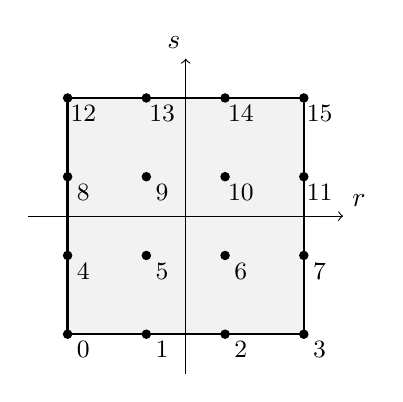
\begin{tikzpicture}
%\draw[step=0.5cm,gray,very thin] (0,0) grid (5,5); 
\draw[fill=gray!10,gray!10](1,1) rectangle (4,4);
\draw[thick] (1,1)--(4,1)--(4,4)--(1,4)--cycle;
\draw [->] (0.5,2.5) -- (4.5,2.5);
\draw [->] (2.5,0.5) -- (2.5,4.5);
\node[] at (4.7,2.7) {$r$};
\node[] at (2.35,4.7) {$s$};
\draw[black,fill=black] (1,1)   circle (1.5pt);
\draw[black,fill=black] (1,2)   circle (1.5pt);
\draw[black,fill=black] (1,3)   circle (1.5pt);
\draw[black,fill=black] (1,4)   circle (1.5pt);
\draw[black,fill=black] (2,1)   circle (1.5pt);
\draw[black,fill=black] (2,2)   circle (1.5pt);
\draw[black,fill=black] (2,3)   circle (1.5pt);
\draw[black,fill=black] (2,4)   circle (1.5pt);
\draw[black,fill=black] (3,1)   circle (1.5pt);
\draw[black,fill=black] (3,2)   circle (1.5pt);
\draw[black,fill=black] (3,3)   circle (1.5pt);
\draw[black,fill=black] (3,4)   circle (1.5pt);
\draw[black,fill=black] (4,1)   circle (1.5pt);
\draw[black,fill=black] (4,2)   circle (1.5pt);
\draw[black,fill=black] (4,3)   circle (1.5pt);
\draw[black,fill=black] (4,4)   circle (1.5pt);
\node[] at (1.2,0.8) {\small $0$};
\node[] at (2.2,0.8) {\small $1$};
\node[] at (3.2,0.8) {\small $2$};
\node[] at (4.2,0.8) {\small $3$};
\node[] at (1.2,1.8) {\small $4$};
\node[] at (2.2,1.8) {\small $5$};
\node[] at (3.2,1.8) {\small $6$};
\node[] at (4.2,1.8) {\small $7$};
\node[] at (1.2,2.8) {\small $8$};
\node[] at (2.2,2.8) {\small $9$};
\node[] at (3.2,2.8) {\small $10$};
\node[] at (4.2,2.8) {\small $11$};
\node[] at (1.2,3.8) {\small $12$};
\node[] at (2.2,3.8) {\small $13$};
\node[] at (3.2,3.8) {\small $14$};
\node[] at (4.2,3.8) {\small $15$};
\end{tikzpicture}
\end{center}

